% Presentación de la defensa final. Regla orientativa: 1 diapositiva por
% minuto de exposición. Las notas para el orador van en \note{...}.
\documentclass[aspectratio=169, 10pt]{beamer}
% Estilo común de las presentaciones. Los datos (título, autor…) salen
% de ../memoria/config/datos.tex, igual que en la memoria.
% =====================================================================
%  DATOS DEL TRABAJO
%  Es el ÚNICO fichero que hay que editar al empezar. Todo lo demás
%  (portada, metadatos del PDF, presentaciones, nombre de los
%  entregables generados por la CI) se alimenta de estas macros.
% =====================================================================

% --- Tipo de trabajo -------------------------------------------------
\newcommand{\TipoTrabajo}{Trabajo Fin de Grado}      % o: Trabajo Fin de Máster
\newcommand{\TipoCorto}{TFG}                         % o: TFM
\newcommand{\Titulacion}{Grado en Ingeniería en Tecnologías Industriales}

% --- Título (español e inglés) ---------------------------------------
\newcommand{\Titulo}{Título del trabajo en español}
\newcommand{\TituloEN}{Project title in English}

% --- Personas ---------------------------------------------------------
\newcommand{\Autor}{Nombre Apellido1 Apellido2}
\newcommand{\Director}{Nombre Apellido1 Apellido2}
\newcommand{\Codirector}{}                           % dejar vacío si no hay

% --- Institución ------------------------------------------------------
\newcommand{\Universidad}{Universidad Pontificia Comillas}
\newcommand{\Escuela}{Escuela Técnica Superior de Ingeniería (ICAI)}
\newcommand{\LogoUniversidad}{figuras/logo_universidad}

% --- Fechas -----------------------------------------------------------
\newcommand{\Lugar}{Madrid}
\newcommand{\FechaEntrega}{Junio 2027}
\newcommand{\CursoAcademico}{2026-2027}

% --- Palabras clave -----------------------------------------------------
\newcommand{\PalabrasClave}{palabra 1, palabra 2, palabra 3, palabra 4}
\newcommand{\Keywords}{keyword 1, keyword 2, keyword 3, keyword 4}

% --- Entrega ----------------------------------------------------------
% Nombre base de los PDF que publica la CI (sin espacios ni tildes).
% Convención: <TIPO>_<Apellido1><Apellido2>_<Nombre>
\newcommand{\NombreEntrega}{TFG_Apellido1Apellido2_Nombre}

% Anexo I (declaración de originalidad, uso de IA y autorización del
% director). La normativa exige: portada -> Anexo I firmado -> portada.
% Poner \AnexoItrue cuando el PDF firmado esté en la ruta indicada.
\newif\ifAnexoI
\AnexoIfalse
\newcommand{\RutaAnexoI}{administrativo/AnexoI_firmado.pdf}


\usepackage[utf8]{inputenc}
\usepackage[T1]{fontenc}
\usepackage[spanish, es-tabla, es-noshorthands]{babel}
\usepackage{etoolbox}
\usepackage{booktabs}
\usepackage{siunitx}
\sisetup{output-decimal-marker={,}}
\usepackage{tikz}
\usetikzlibrary{arrows.meta, positioning}

% Reutiliza las figuras de la memoria sin duplicarlas
\graphicspath{{../memoria/}{../memoria/figuras/}}

% metropolis usa Fira con XeLaTeX/LuaLaTeX; con pdflatex cae a la fuente
% por defecto sin problema, así que se silencia ese aviso.
\usepackage{silence}
\WarningFilter{beamerthememetropolis}{You need to compile with XeLaTeX}
\usetheme{metropolis}
\metroset{progressbar=frametitle, numbering=fraction, block=fill}
\definecolor{acento}{HTML}{1E3A5F}
\setbeamercolor{frametitle}{bg=acento}
\setbeamercolor{progress bar}{fg=acento!60}
\setbeamercolor{alerted text}{fg=acento!80!red}

\title{\Titulo}
\author{\texorpdfstring{\Autor\\{\small Director: \Director\ifdefempty{\Codirector}{}{ · Codirector: \Codirector}}}{\Autor}}
\institute{\footnotesize \TipoTrabajo · \Titulacion\\\Escuela · \Universidad}
% Logo en la esquina de la portada (con tikz para no descuadrar la página)
\usetikzlibrary{calc}
\addtobeamertemplate{title page}{}{%
  \begin{tikzpicture}[remember picture, overlay]
    \node[anchor=north east] at ($(current page.north east)+(-0.5,-0.4)$)
      {\includegraphics[height=1.1cm]{\LogoUniversidad}};
  \end{tikzpicture}}

\date{\Lugar, \FechaEntrega}

\begin{document}

\maketitle

\begin{frame}{Índice}
  \setbeamertemplate{section in toc}[sections numbered]
  \tableofcontents
\end{frame}

\section{Motivación}
\begin{frame}{Contexto y motivación}
  \begin{itemize}
    \item ¿Qué problema se resuelve?
    \item ¿Por qué importa?
  \end{itemize}
  \note{[~60 s] Idea clave que el tribunal debe recordar.}
\end{frame}

\section{Objetivos}
\begin{frame}{Objetivos}
  \begin{enumerate}
    \item \ldots
  \end{enumerate}
\end{frame}

\section{Desarrollo}
\begin{frame}{Solución propuesta}
  \centering
  \begin{tikzpicture}[node distance=1.2cm,
      b/.style={draw, rounded corners, fill=acento!10, minimum width=2.4cm, minimum height=0.9cm}]
    \node[b] (a) {Adquisición};
    \node[b, right=of a] (p) {Procesado};
    \node[b, right=of p] (s) {Visualización};
    \draw[-Stealth, thick] (a) -- (p);
    \draw[-Stealth, thick] (p) -- (s);
  \end{tikzpicture}
\end{frame}

\section{Resultados}
\begin{frame}{Resultados principales}
  \begin{columns}[c]
    \begin{column}{0.58\textwidth}
      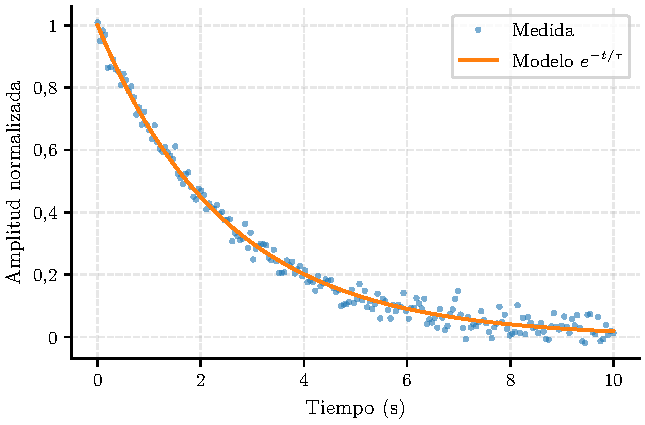
\includegraphics[width=\linewidth]{generadas/ejemplo_curva}
    \end{column}
    \begin{column}{0.4\textwidth}
      \begin{itemize}
        \item Mensaje 1 con una cifra concreta: \qty{3.9}{\percent}
        \item Mensaje 2
      \end{itemize}
    \end{column}
  \end{columns}
\end{frame}

\section{Conclusiones}
\begin{frame}{Conclusiones y trabajo futuro}
  \begin{itemize}
    \item Conclusión 1
    \item Línea futura 1
  \end{itemize}
\end{frame}

\begin{frame}[standout]
  ¡Gracias!\\[1em]
  {\normalsize ¿Preguntas?}
\end{frame}

\end{document}
